% Options for packages loaded elsewhere
\PassOptionsToPackage{unicode}{hyperref}
\PassOptionsToPackage{hyphens}{url}
\PassOptionsToPackage{dvipsnames,svgnames,x11names}{xcolor}
%
\documentclass[
  letterpaper,
  DIV=11,
  numbers=noendperiod]{scrreprt}

\usepackage{amsmath,amssymb}
\usepackage{iftex}
\ifPDFTeX
  \usepackage[T1]{fontenc}
  \usepackage[utf8]{inputenc}
  \usepackage{textcomp} % provide euro and other symbols
\else % if luatex or xetex
  \usepackage{unicode-math}
  \defaultfontfeatures{Scale=MatchLowercase}
  \defaultfontfeatures[\rmfamily]{Ligatures=TeX,Scale=1}
\fi
\usepackage{lmodern}
\ifPDFTeX\else  
    % xetex/luatex font selection
\fi
% Use upquote if available, for straight quotes in verbatim environments
\IfFileExists{upquote.sty}{\usepackage{upquote}}{}
\IfFileExists{microtype.sty}{% use microtype if available
  \usepackage[]{microtype}
  \UseMicrotypeSet[protrusion]{basicmath} % disable protrusion for tt fonts
}{}
\makeatletter
\@ifundefined{KOMAClassName}{% if non-KOMA class
  \IfFileExists{parskip.sty}{%
    \usepackage{parskip}
  }{% else
    \setlength{\parindent}{0pt}
    \setlength{\parskip}{6pt plus 2pt minus 1pt}}
}{% if KOMA class
  \KOMAoptions{parskip=half}}
\makeatother
\usepackage{xcolor}
\setlength{\emergencystretch}{3em} % prevent overfull lines
\setcounter{secnumdepth}{5}
% Make \paragraph and \subparagraph free-standing
\makeatletter
\ifx\paragraph\undefined\else
  \let\oldparagraph\paragraph
  \renewcommand{\paragraph}{
    \@ifstar
      \xxxParagraphStar
      \xxxParagraphNoStar
  }
  \newcommand{\xxxParagraphStar}[1]{\oldparagraph*{#1}\mbox{}}
  \newcommand{\xxxParagraphNoStar}[1]{\oldparagraph{#1}\mbox{}}
\fi
\ifx\subparagraph\undefined\else
  \let\oldsubparagraph\subparagraph
  \renewcommand{\subparagraph}{
    \@ifstar
      \xxxSubParagraphStar
      \xxxSubParagraphNoStar
  }
  \newcommand{\xxxSubParagraphStar}[1]{\oldsubparagraph*{#1}\mbox{}}
  \newcommand{\xxxSubParagraphNoStar}[1]{\oldsubparagraph{#1}\mbox{}}
\fi
\makeatother

\usepackage{color}
\usepackage{fancyvrb}
\newcommand{\VerbBar}{|}
\newcommand{\VERB}{\Verb[commandchars=\\\{\}]}
\DefineVerbatimEnvironment{Highlighting}{Verbatim}{commandchars=\\\{\}}
% Add ',fontsize=\small' for more characters per line
\usepackage{framed}
\definecolor{shadecolor}{RGB}{241,243,245}
\newenvironment{Shaded}{\begin{snugshade}}{\end{snugshade}}
\newcommand{\AlertTok}[1]{\textcolor[rgb]{0.68,0.00,0.00}{#1}}
\newcommand{\AnnotationTok}[1]{\textcolor[rgb]{0.37,0.37,0.37}{#1}}
\newcommand{\AttributeTok}[1]{\textcolor[rgb]{0.40,0.45,0.13}{#1}}
\newcommand{\BaseNTok}[1]{\textcolor[rgb]{0.68,0.00,0.00}{#1}}
\newcommand{\BuiltInTok}[1]{\textcolor[rgb]{0.00,0.23,0.31}{#1}}
\newcommand{\CharTok}[1]{\textcolor[rgb]{0.13,0.47,0.30}{#1}}
\newcommand{\CommentTok}[1]{\textcolor[rgb]{0.37,0.37,0.37}{#1}}
\newcommand{\CommentVarTok}[1]{\textcolor[rgb]{0.37,0.37,0.37}{\textit{#1}}}
\newcommand{\ConstantTok}[1]{\textcolor[rgb]{0.56,0.35,0.01}{#1}}
\newcommand{\ControlFlowTok}[1]{\textcolor[rgb]{0.00,0.23,0.31}{\textbf{#1}}}
\newcommand{\DataTypeTok}[1]{\textcolor[rgb]{0.68,0.00,0.00}{#1}}
\newcommand{\DecValTok}[1]{\textcolor[rgb]{0.68,0.00,0.00}{#1}}
\newcommand{\DocumentationTok}[1]{\textcolor[rgb]{0.37,0.37,0.37}{\textit{#1}}}
\newcommand{\ErrorTok}[1]{\textcolor[rgb]{0.68,0.00,0.00}{#1}}
\newcommand{\ExtensionTok}[1]{\textcolor[rgb]{0.00,0.23,0.31}{#1}}
\newcommand{\FloatTok}[1]{\textcolor[rgb]{0.68,0.00,0.00}{#1}}
\newcommand{\FunctionTok}[1]{\textcolor[rgb]{0.28,0.35,0.67}{#1}}
\newcommand{\ImportTok}[1]{\textcolor[rgb]{0.00,0.46,0.62}{#1}}
\newcommand{\InformationTok}[1]{\textcolor[rgb]{0.37,0.37,0.37}{#1}}
\newcommand{\KeywordTok}[1]{\textcolor[rgb]{0.00,0.23,0.31}{\textbf{#1}}}
\newcommand{\NormalTok}[1]{\textcolor[rgb]{0.00,0.23,0.31}{#1}}
\newcommand{\OperatorTok}[1]{\textcolor[rgb]{0.37,0.37,0.37}{#1}}
\newcommand{\OtherTok}[1]{\textcolor[rgb]{0.00,0.23,0.31}{#1}}
\newcommand{\PreprocessorTok}[1]{\textcolor[rgb]{0.68,0.00,0.00}{#1}}
\newcommand{\RegionMarkerTok}[1]{\textcolor[rgb]{0.00,0.23,0.31}{#1}}
\newcommand{\SpecialCharTok}[1]{\textcolor[rgb]{0.37,0.37,0.37}{#1}}
\newcommand{\SpecialStringTok}[1]{\textcolor[rgb]{0.13,0.47,0.30}{#1}}
\newcommand{\StringTok}[1]{\textcolor[rgb]{0.13,0.47,0.30}{#1}}
\newcommand{\VariableTok}[1]{\textcolor[rgb]{0.07,0.07,0.07}{#1}}
\newcommand{\VerbatimStringTok}[1]{\textcolor[rgb]{0.13,0.47,0.30}{#1}}
\newcommand{\WarningTok}[1]{\textcolor[rgb]{0.37,0.37,0.37}{\textit{#1}}}

\providecommand{\tightlist}{%
  \setlength{\itemsep}{0pt}\setlength{\parskip}{0pt}}\usepackage{longtable,booktabs,array}
\usepackage{calc} % for calculating minipage widths
% Correct order of tables after \paragraph or \subparagraph
\usepackage{etoolbox}
\makeatletter
\patchcmd\longtable{\par}{\if@noskipsec\mbox{}\fi\par}{}{}
\makeatother
% Allow footnotes in longtable head/foot
\IfFileExists{footnotehyper.sty}{\usepackage{footnotehyper}}{\usepackage{footnote}}
\makesavenoteenv{longtable}
\usepackage{graphicx}
\makeatletter
\newsavebox\pandoc@box
\newcommand*\pandocbounded[1]{% scales image to fit in text height/width
  \sbox\pandoc@box{#1}%
  \Gscale@div\@tempa{\textheight}{\dimexpr\ht\pandoc@box+\dp\pandoc@box\relax}%
  \Gscale@div\@tempb{\linewidth}{\wd\pandoc@box}%
  \ifdim\@tempb\p@<\@tempa\p@\let\@tempa\@tempb\fi% select the smaller of both
  \ifdim\@tempa\p@<\p@\scalebox{\@tempa}{\usebox\pandoc@box}%
  \else\usebox{\pandoc@box}%
  \fi%
}
% Set default figure placement to htbp
\def\fps@figure{htbp}
\makeatother
% definitions for citeproc citations
\NewDocumentCommand\citeproctext{}{}
\NewDocumentCommand\citeproc{mm}{%
  \begingroup\def\citeproctext{#2}\cite{#1}\endgroup}
\makeatletter
 % allow citations to break across lines
 \let\@cite@ofmt\@firstofone
 % avoid brackets around text for \cite:
 \def\@biblabel#1{}
 \def\@cite#1#2{{#1\if@tempswa , #2\fi}}
\makeatother
\newlength{\cslhangindent}
\setlength{\cslhangindent}{1.5em}
\newlength{\csllabelwidth}
\setlength{\csllabelwidth}{3em}
\newenvironment{CSLReferences}[2] % #1 hanging-indent, #2 entry-spacing
 {\begin{list}{}{%
  \setlength{\itemindent}{0pt}
  \setlength{\leftmargin}{0pt}
  \setlength{\parsep}{0pt}
  % turn on hanging indent if param 1 is 1
  \ifodd #1
   \setlength{\leftmargin}{\cslhangindent}
   \setlength{\itemindent}{-1\cslhangindent}
  \fi
  % set entry spacing
  \setlength{\itemsep}{#2\baselineskip}}}
 {\end{list}}
\usepackage{calc}
\newcommand{\CSLBlock}[1]{\hfill\break\parbox[t]{\linewidth}{\strut\ignorespaces#1\strut}}
\newcommand{\CSLLeftMargin}[1]{\parbox[t]{\csllabelwidth}{\strut#1\strut}}
\newcommand{\CSLRightInline}[1]{\parbox[t]{\linewidth - \csllabelwidth}{\strut#1\strut}}
\newcommand{\CSLIndent}[1]{\hspace{\cslhangindent}#1}

\KOMAoption{captions}{tableheading}
\makeatletter
\@ifpackageloaded{bookmark}{}{\usepackage{bookmark}}
\makeatother
\makeatletter
\@ifpackageloaded{caption}{}{\usepackage{caption}}
\AtBeginDocument{%
\ifdefined\contentsname
  \renewcommand*\contentsname{Table of contents}
\else
  \newcommand\contentsname{Table of contents}
\fi
\ifdefined\listfigurename
  \renewcommand*\listfigurename{List of Figures}
\else
  \newcommand\listfigurename{List of Figures}
\fi
\ifdefined\listtablename
  \renewcommand*\listtablename{List of Tables}
\else
  \newcommand\listtablename{List of Tables}
\fi
\ifdefined\figurename
  \renewcommand*\figurename{Figure}
\else
  \newcommand\figurename{Figure}
\fi
\ifdefined\tablename
  \renewcommand*\tablename{Table}
\else
  \newcommand\tablename{Table}
\fi
}
\@ifpackageloaded{float}{}{\usepackage{float}}
\floatstyle{ruled}
\@ifundefined{c@chapter}{\newfloat{codelisting}{h}{lop}}{\newfloat{codelisting}{h}{lop}[chapter]}
\floatname{codelisting}{Listing}
\newcommand*\listoflistings{\listof{codelisting}{List of Listings}}
\makeatother
\makeatletter
\makeatother
\makeatletter
\@ifpackageloaded{caption}{}{\usepackage{caption}}
\@ifpackageloaded{subcaption}{}{\usepackage{subcaption}}
\makeatother

\usepackage{bookmark}

\IfFileExists{xurl.sty}{\usepackage{xurl}}{} % add URL line breaks if available
\urlstyle{same} % disable monospaced font for URLs
\hypersetup{
  pdftitle={Panduan Sederhana Git dan Github},
  pdfauthor={Norah Jones},
  colorlinks=true,
  linkcolor={blue},
  filecolor={Maroon},
  citecolor={Blue},
  urlcolor={Blue},
  pdfcreator={LaTeX via pandoc}}


\title{Panduan Sederhana Git dan Github}
\author{Norah Jones}
\date{2025-02-13}

\begin{document}
\maketitle

\renewcommand*\contentsname{Table of contents}
{
\hypersetup{linkcolor=}
\setcounter{tocdepth}{2}
\tableofcontents
}

\bookmarksetup{startatroot}

\chapter*{Preface}\label{preface}
\addcontentsline{toc}{chapter}{Preface}

\markboth{Preface}{Preface}

Dalam berkreasi menghasilkan tulisan, paper, disertasi, konten, software
kita sering menghadapi kebingungan, kelelahan, dan kebuntuan akibat
sifat kompleksitas yang tinggi.

Berbagai alat bantu digital telah sangat menolong, tetapi ancaman
kompleksitas selalu mengancam. Akibatnya kalaupun tugas ini selesai,
kualitas tidak maksimal, waktu terlalu lama, dan biaya yang dikeluarkan
membengkak.

Jalan keluarnya adalah dengan menguraikan pekerjaan ke dalam potongan,
tahapan, untuk dikrjakan sendiri atau parlelisasi.

Git dan Github alat digital yang sangat berguna untuk mengelola berbagai
potongan pekerjaan dan mendistribusinya pada banyak orang, dengan tetap
menjaga integritas proyek.

Git mengendalikan pnguraian pekerjaan ke dalam potongan-potongan
penugasan, mencatat siapa yang mengambil potongan pekerjaan tertentu,
lalu memantau penyelesaiainya. Pekerjaan juga dapat diurai ke dalam
versi-versi, sehingga sebelum pengembangan versi baru selesai versi lama
tetap tersedia.

Git mengenal tiga tempat penyimpanan: lokal repository, staging, dan
working space.

Adapun Github menjadi pusat distribusi, sehingga Github menyimpan
repositori utama (master atau main) dan setiap individu kontributor
memiliki replikasi dari repositori master, yaitu replikasi lokal.

Sebagaimana diperlihatkan pada Gambar Figure~\ref{fig-git-github},
Github menjdi pusat dari banyak kontributor dengan repositori lokal
masing masing. Git dan Github bekerjasama mengatur potongan mana yang
dikerjakan kontributor tertentu, dan mencegah tumpang tindih atau
pengerjaan bagian sama pada saat yang sama oleh kntributor yang berbeda.

\begin{figure}

\centering{

\pandocbounded{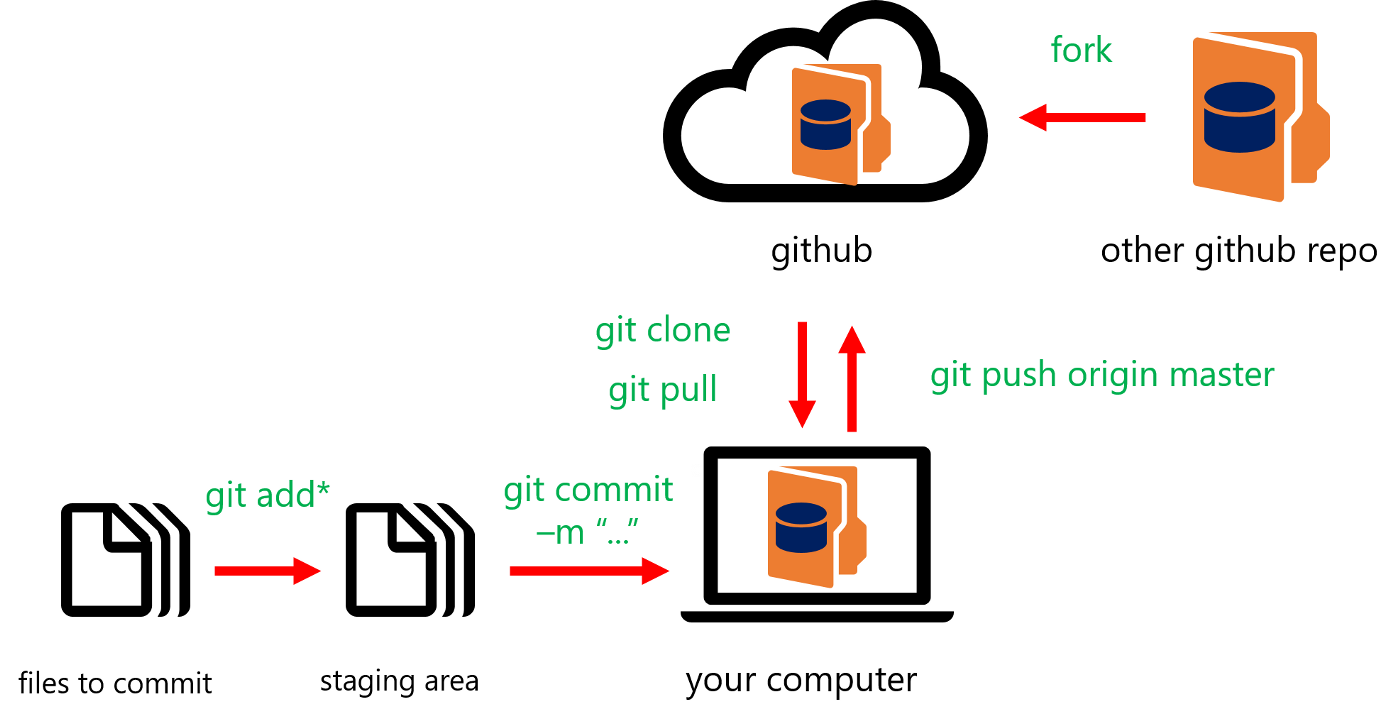
\includegraphics[keepaspectratio]{images/gitgithub.png}}

}

\caption{\label{fig-git-github}Git dan Github}

\end{figure}%

Dari gambar ini, dapat dimengerti bahwa kontributor bekerja di working
space, yang bila hasinya memuaskan, di kirim ke staging area (yang
biasanya hidden dari kontrbutor ) untuk menunggu keputusan apakah hendak
di commit ke local repository. Untuk proyek personal, proses berhenti
cukup di sini

Bila diputuskan untuk untuk masuk ke repository utama, maka proses push
diinisiasi, yang biasanya diterima kecuali bisa ada anomali seperti
duplikasi kntributor tadi.

Mengingat pentingnya mengkombinasi personalisasi kontribusi (git) dan
kolaborasi (Github) maka dipandang perlu akadmisi memanfaatkan alat
bantu ini. Untuk itu tulisan ini dibuat.

Proses pembuatan tulisan ini menggunakan Git dan sedikit Github. Tulisan
ini dibuat menggunakan texteditor, dengan format markdwon versi Quarto

Bandung, 13 Februari 2025 Armein Z R Langi

\bookmarksetup{startatroot}

\chapter{Git dan Github}\label{git-dan-github}

\subsection{\texorpdfstring{📌 \textbf{Konsep Dasar
Git}}{📌 Konsep Dasar Git}}\label{konsep-dasar-git}

\textbf{Git} adalah sistem kontrol versi (VCS) terdistribusi yang
digunakan untuk melacak perubahan dalam kode, memungkinkan kolaborasi,
dan mengelola proyek perangkat lunak dengan lebih efisien.

\begin{center}\rule{0.5\linewidth}{0.5pt}\end{center}

\section{\texorpdfstring{🔹 \textbf{1. Apa Itu
Git?}}{🔹 1. Apa Itu Git?}}\label{apa-itu-git}

Git adalah alat yang memungkinkan: - \textbf{Versi Kontrol}: Melacak
perubahan kode dari waktu ke waktu. - \textbf{Kolaborasi}: Memungkinkan
banyak orang bekerja di proyek yang sama tanpa konflik. -
\textbf{Distribusi}: Setiap pengembang memiliki salinan lengkap dari
repositori.

\begin{center}\rule{0.5\linewidth}{0.5pt}\end{center}

\section{\texorpdfstring{🔹 \textbf{2. Arsitektur \& Cara Kerja
Git}}{🔹 2. Arsitektur \& Cara Kerja Git}}\label{arsitektur-cara-kerja-git}

Git memiliki tiga area utama:

\begin{longtable}[]{@{}
  >{\raggedright\arraybackslash}p{(\linewidth - 2\tabcolsep) * \real{0.4545}}
  >{\raggedright\arraybackslash}p{(\linewidth - 2\tabcolsep) * \real{0.5455}}@{}}
\toprule\noalign{}
\begin{minipage}[b]{\linewidth}\raggedright
\textbf{Area}
\end{minipage} & \begin{minipage}[b]{\linewidth}\raggedright
\textbf{Fungsi}
\end{minipage} \\
\midrule\noalign{}
\endhead
\bottomrule\noalign{}
\endlastfoot
\textbf{Working Directory} & Tempat di mana file saat ini diedit. \\
\textbf{Staging Area} & Area persiapan sebelum file dikomit. \\
\textbf{Repository (Local Repo)} & Tempat penyimpanan perubahan yang
telah dikomit. \\
\textbf{Remote Repository} & Repositori yang disimpan di server (GitHub,
GitLab, dll.). \\
\end{longtable}

⚡ \textbf{Alur Kerja Git:} 1. \textbf{Edit File} → di \textbf{Working
Directory}. 2. \textbf{Tambah ke Staging Area} →
\texttt{git\ add\ file.txt} 3. \textbf{Commit ke Repository} →
\texttt{git\ commit\ -m\ "Pesan\ commit"} 4. \textbf{Push ke Remote
Repo} → \texttt{git\ push\ origin\ main}

\begin{center}\rule{0.5\linewidth}{0.5pt}\end{center}

\section{\texorpdfstring{🔹 \textbf{3. Perintah Dasar
Git}}{🔹 3. Perintah Dasar Git}}\label{perintah-dasar-git}

\begin{longtable}[]{@{}ll@{}}
\toprule\noalign{}
Perintah & Fungsi \\
\midrule\noalign{}
\endhead
\bottomrule\noalign{}
\endlastfoot
\texttt{git\ init} & Membuat repositori Git baru. \\
\texttt{git\ clone\ URL} & Mengunduh repositori dari remote. \\
\texttt{git\ add\ file.txt} & Menambahkan file ke staging area. \\
\texttt{git\ commit\ -m\ "Pesan"} & Menyimpan perubahan ke repositori
lokal. \\
\texttt{git\ push\ origin\ main} & Mengunggah perubahan ke repositori
remote. \\
\texttt{git\ pull\ origin\ main} & Mengambil perubahan terbaru dari
remote. \\
\texttt{git\ status} & Melihat status perubahan file. \\
\texttt{git\ log} & Melihat riwayat commit. \\
\texttt{git\ branch\ feature-X} & Membuat branch baru. \\
\texttt{git\ checkout\ feature-X} & Berpindah ke branch lain. \\
\texttt{git\ merge\ feature-X} & Menggabungkan branch ke branch
utama. \\
\end{longtable}

\begin{center}\rule{0.5\linewidth}{0.5pt}\end{center}

\section{\texorpdfstring{🔹 \textbf{4. Branching \&
Merging}}{🔹 4. Branching \& Merging}}\label{branching-merging}

Git memungkinkan pengembang bekerja di fitur yang berbeda tanpa
mengganggu kode utama.

\begin{enumerate}
\def\labelenumi{\arabic{enumi}.}
\tightlist
\item
  \textbf{Membuat branch baru} → \texttt{git\ branch\ feature-1}
\item
  \textbf{Beralih ke branch} → \texttt{git\ checkout\ feature-1}
\item
  \textbf{Edit \& commit perubahan} →
  \texttt{git\ commit\ -m\ "Tambah\ fitur"}
\item
  \textbf{Kembali ke branch utama} → \texttt{git\ checkout\ main}
\item
  \textbf{Gabungkan branch} → \texttt{git\ merge\ feature-1}
\end{enumerate}

\textbf{🔀 Git Flow Umum:} - \textbf{\texttt{main}} → Branch stabil
(production). - \textbf{\texttt{develop}} → Branch pengembangan utama. -
\textbf{Feature Branches} → Untuk fitur baru, lalu digabungkan ke
\texttt{develop}.

\begin{center}\rule{0.5\linewidth}{0.5pt}\end{center}

\section{\texorpdfstring{🔹 \textbf{5. Remote Repository (GitHub,
GitLab,
Bitbucket)}}{🔹 5. Remote Repository (GitHub, GitLab, Bitbucket)}}\label{remote-repository-github-gitlab-bitbucket}

Git dapat terhubung ke layanan cloud seperti \textbf{GitHub} untuk
kolaborasi.

\begin{enumerate}
\def\labelenumi{\arabic{enumi}.}
\item
  \textbf{Tambahkan Remote Repo}:

\begin{verbatim}
git remote add origin https://github.com/user/repo.git
\end{verbatim}
\item
  \textbf{Push kode ke GitHub}:

\begin{verbatim}
git push -u origin main
\end{verbatim}
\item
  \textbf{Ambil perubahan dari GitHub}:

\begin{verbatim}
git pull origin main
\end{verbatim}
\end{enumerate}

\begin{center}\rule{0.5\linewidth}{0.5pt}\end{center}

\section{\texorpdfstring{🎯
\textbf{Kesimpulan}}{🎯 Kesimpulan}}\label{kesimpulan}

\begin{itemize}
\tightlist
\item
  \textbf{Git membantu dalam pengelolaan kode secara terstruktur.}
\item
  \textbf{Memungkinkan banyak pengembang bekerja di proyek yang sama.}
\item
  \textbf{Branching mempermudah pengembangan fitur tanpa mengganggu kode
  utama.}
\item
  \textbf{Remote repository (seperti GitHub) membuat kolaborasi lebih
  mudah.}
\end{itemize}

➡ \textbf{Ada bagian yang ingin kamu eksplor lebih dalam?} 🚀

\bookmarksetup{startatroot}

\chapter{Contoh Praktis}\label{contoh-praktis}

\subsection{\texorpdfstring{📌 \textbf{Contoh Realistis Proyek Pembuatan
Software di Linux dengan
Git}}{📌 Contoh Realistis Proyek Pembuatan Software di Linux dengan Git}}\label{contoh-realistis-proyek-pembuatan-software-di-linux-dengan-git}

Kita akan membuat proyek software sederhana bernama \textbf{``MyApp''},
sebuah program CLI yang ditulis dalam \textbf{Python}. Proyek ini akan
menggunakan \textbf{Git} untuk mengelola versi dan berkolaborasi.

\begin{center}\rule{0.5\linewidth}{0.5pt}\end{center}

\section{\texorpdfstring{🔹 \textbf{1. Inisialisasi
Proyek}}{🔹 1. Inisialisasi Proyek}}\label{inisialisasi-proyek}

\subsection{\texorpdfstring{🔥 \textbf{Langkah 1: Buat Direktori
Proyek}}{🔥 Langkah 1: Buat Direktori Proyek}}\label{langkah-1-buat-direktori-proyek}

Di terminal Linux, jalankan:

\begin{Shaded}
\begin{Highlighting}[]
\FunctionTok{mkdir}\NormalTok{ MyApp}
\BuiltInTok{cd}\NormalTok{ MyApp}
\end{Highlighting}
\end{Shaded}

\subsection{\texorpdfstring{🔥 \textbf{Langkah 2: Inisialisasi
Git}}{🔥 Langkah 2: Inisialisasi Git}}\label{langkah-2-inisialisasi-git}

\begin{Shaded}
\begin{Highlighting}[]
\FunctionTok{git}\NormalTok{ init}
\end{Highlighting}
\end{Shaded}

📌 \textbf{Git akan membuat repositori kosong di dalam folder proyek.}

\begin{center}\rule{0.5\linewidth}{0.5pt}\end{center}

\section{\texorpdfstring{🔹 \textbf{2. Menambahkan File
Awal}}{🔹 2. Menambahkan File Awal}}\label{menambahkan-file-awal}

\subsection{\texorpdfstring{🔥 \textbf{Langkah 3: Buat File Program
Utama}}{🔥 Langkah 3: Buat File Program Utama}}\label{langkah-3-buat-file-program-utama}

Buat file \texttt{app.py}:

\begin{Shaded}
\begin{Highlighting}[]
\FunctionTok{touch}\NormalTok{ app.py}
\end{Highlighting}
\end{Shaded}

Edit \texttt{app.py}:

\begin{Shaded}
\begin{Highlighting}[]
\BuiltInTok{print}\NormalTok{(}\StringTok{"Hello, this is MyApp!"}\NormalTok{)}
\end{Highlighting}
\end{Shaded}

\subsection{\texorpdfstring{🔥 \textbf{Langkah 4: Tambahkan
README}}{🔥 Langkah 4: Tambahkan README}}\label{langkah-4-tambahkan-readme}

\begin{Shaded}
\begin{Highlighting}[]
\BuiltInTok{echo} \StringTok{"\# MyApp"} \OperatorTok{\textgreater{}}\NormalTok{ README.md}
\end{Highlighting}
\end{Shaded}

\subsection{\texorpdfstring{🔥 \textbf{Langkah 5: Tambahkan File ke
Git}}{🔥 Langkah 5: Tambahkan File ke Git}}\label{langkah-5-tambahkan-file-ke-git}

\begin{Shaded}
\begin{Highlighting}[]
\FunctionTok{git}\NormalTok{ add app.py README.md}
\end{Highlighting}
\end{Shaded}

📌 \textbf{Perintah \texttt{git\ add} menambahkan file ke Staging Area.}

\subsection{\texorpdfstring{🔥 \textbf{Langkah 6: Commit
Perubahan}}{🔥 Langkah 6: Commit Perubahan}}\label{langkah-6-commit-perubahan}

\begin{Shaded}
\begin{Highlighting}[]
\FunctionTok{git}\NormalTok{ commit }\AttributeTok{{-}m} \StringTok{"Inisialisasi proyek dengan file utama dan README"}
\end{Highlighting}
\end{Shaded}

📌 \textbf{Perintah \texttt{git\ commit} menyimpan perubahan ke dalam
riwayat versi.}

\begin{center}\rule{0.5\linewidth}{0.5pt}\end{center}

\section{\texorpdfstring{🔹 \textbf{3. Menambahkan Remote Repository
(GitHub)}}{🔹 3. Menambahkan Remote Repository (GitHub)}}\label{menambahkan-remote-repository-github}

Sekarang, kita ingin menyimpan proyek ini di GitHub.

\subsection{\texorpdfstring{🔥 \textbf{Langkah 7: Tambahkan Remote
Repository}}{🔥 Langkah 7: Tambahkan Remote Repository}}\label{langkah-7-tambahkan-remote-repository}

\begin{Shaded}
\begin{Highlighting}[]
\FunctionTok{git}\NormalTok{ remote add origin https://github.com/username/MyApp.git}
\end{Highlighting}
\end{Shaded}

📌 \textbf{Gantilah \texttt{username} dengan akun GitHub kamu.}

\subsection{\texorpdfstring{🔥 \textbf{Langkah 8: Push Kode ke
GitHub}}{🔥 Langkah 8: Push Kode ke GitHub}}\label{langkah-8-push-kode-ke-github}

\begin{Shaded}
\begin{Highlighting}[]
\FunctionTok{git}\NormalTok{ push }\AttributeTok{{-}u}\NormalTok{ origin main}
\end{Highlighting}
\end{Shaded}

📌 \textbf{Kode pertama kali diunggah ke GitHub pada branch
\texttt{main}.}

\begin{center}\rule{0.5\linewidth}{0.5pt}\end{center}

\section{\texorpdfstring{🔹 \textbf{4. Pengembangan Fitur Baru dengan
Branch}}{🔹 4. Pengembangan Fitur Baru dengan Branch}}\label{pengembangan-fitur-baru-dengan-branch}

Misalnya, kita ingin menambahkan fitur baru: \textbf{menampilkan waktu
saat ini}.

\subsection{\texorpdfstring{🔥 \textbf{Langkah 9: Buat dan Beralih ke
Branch
Baru}}{🔥 Langkah 9: Buat dan Beralih ke Branch Baru}}\label{langkah-9-buat-dan-beralih-ke-branch-baru}

\begin{Shaded}
\begin{Highlighting}[]
\FunctionTok{git}\NormalTok{ branch feature{-}time}
\FunctionTok{git}\NormalTok{ checkout feature{-}time}
\end{Highlighting}
\end{Shaded}

📌 \textbf{Branch \texttt{feature-time} dibuat untuk pengembangan fitur
tanpa mengganggu branch utama.}

\subsection{\texorpdfstring{🔥 \textbf{Langkah 10: Edit \texttt{app.py}
untuk Menampilkan
Waktu}}{🔥 Langkah 10: Edit app.py untuk Menampilkan Waktu}}\label{langkah-10-edit-app.py-untuk-menampilkan-waktu}

Edit \texttt{app.py}:

\begin{Shaded}
\begin{Highlighting}[]
\ImportTok{import}\NormalTok{ datetime}

\BuiltInTok{print}\NormalTok{(}\StringTok{"Hello, this is MyApp!"}\NormalTok{)}
\BuiltInTok{print}\NormalTok{(}\StringTok{"Current Time:"}\NormalTok{, datetime.datetime.now())}
\end{Highlighting}
\end{Shaded}

\subsection{\texorpdfstring{🔥 \textbf{Langkah 11: Commit Perubahan di
Branch
Fitur}}{🔥 Langkah 11: Commit Perubahan di Branch Fitur}}\label{langkah-11-commit-perubahan-di-branch-fitur}

\begin{Shaded}
\begin{Highlighting}[]
\FunctionTok{git}\NormalTok{ add app.py}
\FunctionTok{git}\NormalTok{ commit }\AttributeTok{{-}m} \StringTok{"Menambahkan fitur waktu ke MyApp"}
\end{Highlighting}
\end{Shaded}

\begin{center}\rule{0.5\linewidth}{0.5pt}\end{center}

\section{\texorpdfstring{🔹 \textbf{5. Menggabungkan Fitur ke
\texttt{main}}}{🔹 5. Menggabungkan Fitur ke main}}\label{menggabungkan-fitur-ke-main}

Setelah fitur selesai diuji, kita gabungkan ke branch \texttt{main}.

\subsection{\texorpdfstring{🔥 \textbf{Langkah 12: Pindah ke Branch
\texttt{main}}}{🔥 Langkah 12: Pindah ke Branch main}}\label{langkah-12-pindah-ke-branch-main}

\begin{Shaded}
\begin{Highlighting}[]
\FunctionTok{git}\NormalTok{ checkout main}
\end{Highlighting}
\end{Shaded}

\subsection{\texorpdfstring{🔥 \textbf{Langkah 13: Gabungkan
Fitur}}{🔥 Langkah 13: Gabungkan Fitur}}\label{langkah-13-gabungkan-fitur}

\begin{Shaded}
\begin{Highlighting}[]
\FunctionTok{git}\NormalTok{ merge feature{-}time}
\end{Highlighting}
\end{Shaded}

📌 \textbf{Branch \texttt{feature-time} digabungkan ke \texttt{main}.}

\subsection{\texorpdfstring{🔥 \textbf{Langkah 14: Push Perubahan ke
GitHub}}{🔥 Langkah 14: Push Perubahan ke GitHub}}\label{langkah-14-push-perubahan-ke-github}

\begin{Shaded}
\begin{Highlighting}[]
\FunctionTok{git}\NormalTok{ push origin main}
\end{Highlighting}
\end{Shaded}

📌 \textbf{Kode terbaru sekarang ada di GitHub.}

\begin{center}\rule{0.5\linewidth}{0.5pt}\end{center}

\section{\texorpdfstring{🔹 \textbf{6. Bekerja dengan Tim (Pull Request
dan
Merge)}}{🔹 6. Bekerja dengan Tim (Pull Request dan Merge)}}\label{bekerja-dengan-tim-pull-request-dan-merge}

Jika bekerja dalam tim, biasanya: 1. \textbf{Developer lain membuat
branch fitur baru dan push ke GitHub}:
\texttt{bash\ \ \ \ git\ push\ origin\ feature-time} 2. \textbf{Di
GitHub, developer membuat Pull Request} dan meminta merge ke
\texttt{main}. 3. \textbf{Tim melakukan review kode} dan menyetujui
merge. 4. \textbf{Merge dilakukan di GitHub atau melalui terminal:}
\texttt{bash\ \ \ \ git\ checkout\ main\ \ \ \ git\ pull\ origin\ main}

\begin{center}\rule{0.5\linewidth}{0.5pt}\end{center}

\section{\texorpdfstring{🔹 \textbf{7. Mengelola Bug dan
Revisi}}{🔹 7. Mengelola Bug dan Revisi}}\label{mengelola-bug-dan-revisi}

Misalnya, kita menemukan bug di \texttt{app.py}.

\subsection{\texorpdfstring{🔥 \textbf{Langkah 15: Buat Branch untuk
Perbaikan
Bug}}{🔥 Langkah 15: Buat Branch untuk Perbaikan Bug}}\label{langkah-15-buat-branch-untuk-perbaikan-bug}

\begin{Shaded}
\begin{Highlighting}[]
\FunctionTok{git}\NormalTok{ branch fix{-}bug}
\FunctionTok{git}\NormalTok{ checkout fix{-}bug}
\end{Highlighting}
\end{Shaded}

Edit \texttt{app.py} untuk memperbaiki bug, lalu:

\begin{Shaded}
\begin{Highlighting}[]
\FunctionTok{git}\NormalTok{ add app.py}
\FunctionTok{git}\NormalTok{ commit }\AttributeTok{{-}m} \StringTok{"Memperbaiki bug dalam fitur waktu"}
\FunctionTok{git}\NormalTok{ checkout main}
\FunctionTok{git}\NormalTok{ merge fix{-}bug}
\FunctionTok{git}\NormalTok{ push origin main}
\end{Highlighting}
\end{Shaded}

\begin{center}\rule{0.5\linewidth}{0.5pt}\end{center}

\section{\texorpdfstring{🔹 \textbf{8. Membuat Versi
Rilis}}{🔹 8. Membuat Versi Rilis}}\label{membuat-versi-rilis}

Setelah pengembangan stabil, kita bisa membuat \textbf{versi rilis}.

\subsection{\texorpdfstring{🔥 \textbf{Langkah 16: Buat Tag untuk
Rilis}}{🔥 Langkah 16: Buat Tag untuk Rilis}}\label{langkah-16-buat-tag-untuk-rilis}

\begin{Shaded}
\begin{Highlighting}[]
\FunctionTok{git}\NormalTok{ tag }\AttributeTok{{-}a}\NormalTok{ v1.0 }\AttributeTok{{-}m} \StringTok{"Rilis pertama MyApp"}
\FunctionTok{git}\NormalTok{ push origin v1.0}
\end{Highlighting}
\end{Shaded}

📌 \textbf{Git akan menandai versi \texttt{v1.0} untuk rilis.}

\begin{center}\rule{0.5\linewidth}{0.5pt}\end{center}

\section{\texorpdfstring{🎯
\textbf{Kesimpulan}}{🎯 Kesimpulan}}\label{kesimpulan-1}

\begin{enumerate}
\def\labelenumi{\arabic{enumi}.}
\tightlist
\item
  \textbf{Gunakan Git untuk mengelola proyek dengan aman.}\\
\item
  \textbf{Gunakan branch untuk pengembangan fitur dan perbaikan bug.}\\
\item
  \textbf{Simpan proyek di GitHub untuk kolaborasi dan backup.}\\
\item
  \textbf{Gunakan tagging (\texttt{git\ tag}) untuk merilis versi
  stabil.}
\end{enumerate}

➡ \textbf{Mau coba proyek lain atau ada pertanyaan?} 🚀\# Summary

In summary, this book has no content whatsoever.

\bookmarksetup{startatroot}

\chapter*{References}\label{references}
\addcontentsline{toc}{chapter}{References}

\markboth{References}{References}

\phantomsection\label{refs}
\begin{CSLReferences}{0}{1}
\end{CSLReferences}




\end{document}
